\begin{figure}[t]
\centering
\pgfplotsset{compat=1.18}
\definecolor{cNOOA}{RGB}{31,119,180}    % blue
\definecolor{cBASE}{RGB}{23,165,137}    % teal
\definecolor{cOC}{RGB}{230,126,34}      % orange
\definecolor{cPI}{RGB}{155,89,182}      % purple
% marker size = reasoning effort
\newcommand{\szoff}{1.7}\newcommand{\szhi}{3.2}\newcommand{\szxhi}{4.8}
\newcommand{\sqoff}{1.7}\newcommand{\sqhi}{3.2}
\newcommand{\trioff}{2.1}\newcommand{\trion}{3.9}
\tikzset{lead/.style={gray!55, line width=0.3pt}, lab/.style={font=\scriptsize, inner sep=1pt}}
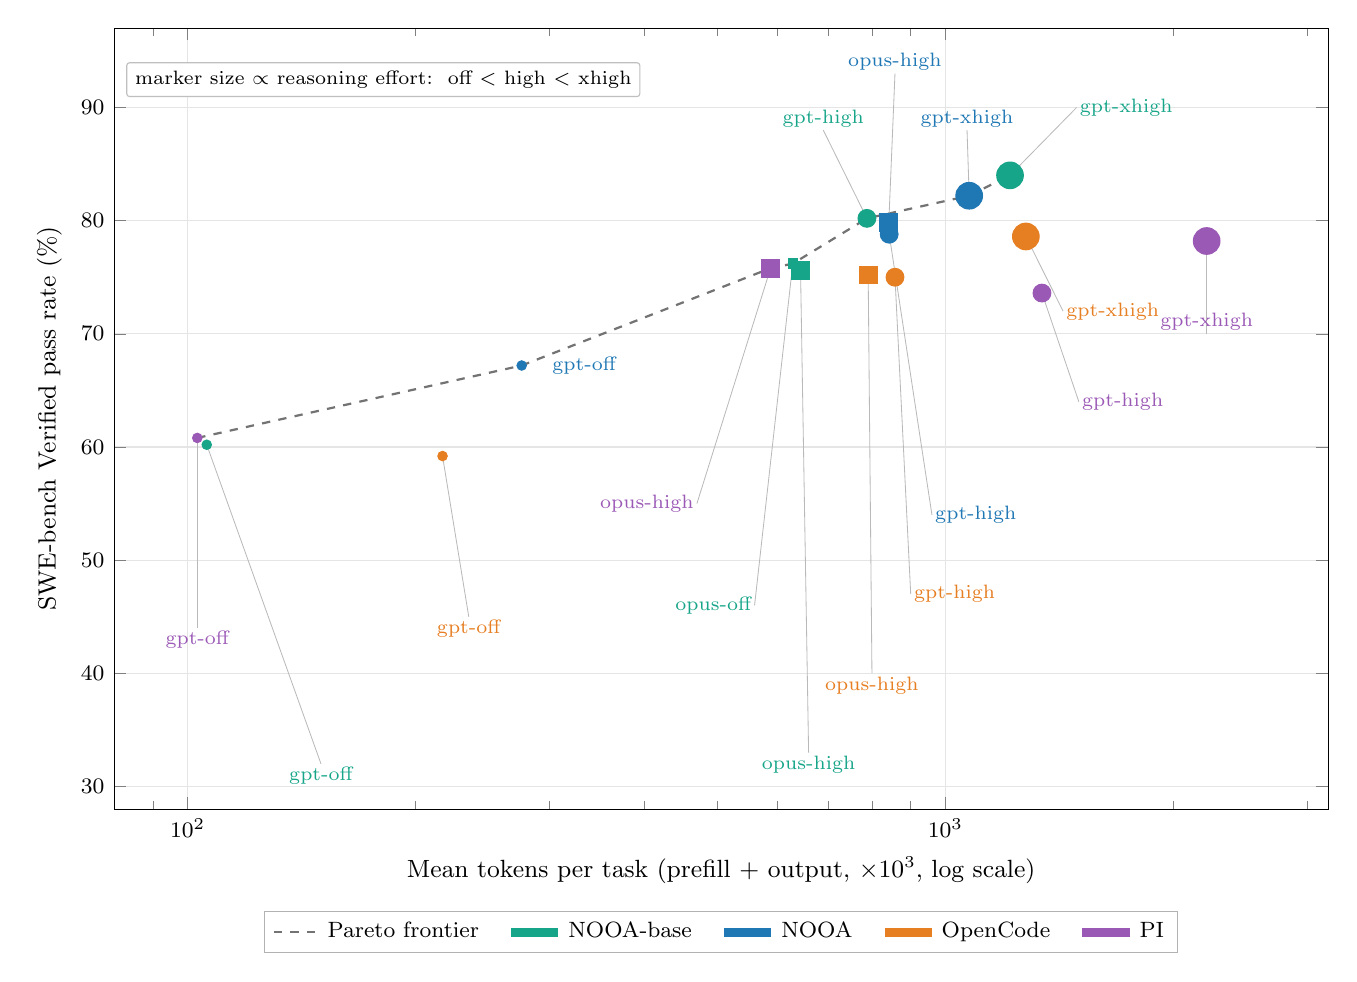
\begin{tikzpicture}
\begin{semilogxaxis}[
  width=17cm, height=11.5cm,
  xlabel={Mean tokens per task (prefill + output, $\times 10^3$, log scale)},
  ylabel={SWE-bench Verified pass rate (\%)},
  xmin=80, xmax=3200, ymin=28, ymax=97,
  grid=major, grid style={black!10},
  legend cell align=left,
  legend style={at={(0.5,-0.13)}, anchor=north, legend columns=5,
    font=\footnotesize, draw=black!30,
    /tikz/every even column/.append style={column sep=8pt}},
  tick label style={font=\footnotesize}, label style={font=\small},
]
%\fill[black!5] (axis cs:80,-2) rectangle (axis cs:3200,25);
\node[anchor=north west, font=\scriptsize, draw=black!25, fill=white,
      rounded corners=1pt, inner sep=3pt] at (axis cs:83,94)
  {marker size $\propto$ reasoning effort:\ \ off $<$ high $<$ xhigh};
\addplot[black!55, dashed, thick, mark=none] coordinates {
  (103,60.8) (276,67.2) (588,75.8) (629,76.2) (788,80.2) (1075,82.2) (1217,84.0)};
\addlegendentry{Pareto frontier}
% ----- leader lines -----
\draw[lead] (axis cs:103,60.8) -- (axis cs:103,44);
\draw[lead] (axis cs:106,60.2) -- (axis cs:150,32);
\draw[lead] (axis cs:217,59.2) -- (axis cs:235,45);
\draw[lead] (axis cs:588,75.8) -- (axis cs:470,55);
\draw[lead] (axis cs:629,76.2) -- (axis cs:560,46);
\draw[lead] (axis cs:644,75.6) -- (axis cs:660,33);
\draw[lead] (axis cs:788,80.2) -- (axis cs:690,88);
\draw[lead] (axis cs:791,75.2) -- (axis cs:800,40);
\draw[lead] (axis cs:842,79.8) -- (axis cs:858,93);
\draw[lead] (axis cs:843,78.8) -- (axis cs:960,54);
\draw[lead] (axis cs:858,75.0) -- (axis cs:900,47);
\draw[lead] (axis cs:1075,82.2) -- (axis cs:1068,88);
\draw[lead] (axis cs:1217,84.0) -- (axis cs:1490,90);
\draw[lead] (axis cs:1277,78.6) -- (axis cs:1430,72);
\draw[lead] (axis cs:1341,73.6) -- (axis cs:1500,64);
\draw[lead] (axis cs:2212,78.2) -- (axis cs:2212,70);
% ----- markers: color=harness, shape=backend, size=effort -----
\addplot[forget plot,only marks,mark=*,        mark size=\szoff pt, cBASE] coordinates {(106,60.2)};
\addplot[forget plot,only marks,mark=*,        mark size=\szhi pt,  cBASE] coordinates {(788,80.2)};
\addplot[forget plot,only marks,mark=*,        mark size=\szxhi pt, cBASE] coordinates {(1217,84.0)};
\addplot[forget plot,only marks,mark=square*,  mark size=\sqoff pt, cBASE] coordinates {(629,76.2)};
\addplot[forget plot,only marks,mark=square*,  mark size=\sqhi pt,  cBASE] coordinates {(644,75.6)};
%\addplot[forget plot,only marks,mark=triangle*,mark size=\trion pt, cBASE] coordinates {(155,3.4)};
%\addplot[forget plot,only marks,mark=triangle*,mark size=\trioff pt,cBASE] coordinates {(396,1.8)};
\addplot[forget plot,only marks,mark=*,        mark size=\szoff pt, cNOOA] coordinates {(276,67.2)};
\addplot[forget plot,only marks,mark=*,        mark size=\szhi pt,  cNOOA] coordinates {(843,78.8)};
\addplot[forget plot,only marks,mark=*,        mark size=\szxhi pt, cNOOA] coordinates {(1075,82.2)};
\addplot[forget plot,only marks,mark=square*,  mark size=\sqhi pt,  cNOOA] coordinates {(842,79.8)};
%\addplot[forget plot,only marks,mark=triangle*,mark size=\trioff pt,cNOOA] coordinates {(1162,6.0)};
%\addplot[forget plot,only marks,mark=triangle*,mark size=\trion pt, cNOOA] coordinates {(1431,16.2)};
\addplot[forget plot,only marks,mark=*,        mark size=\szoff pt, cOC] coordinates {(217,59.2)};
\addplot[forget plot,only marks,mark=*,        mark size=\szhi pt,  cOC] coordinates {(858,75.0)};
\addplot[forget plot,only marks,mark=*,        mark size=\szxhi pt, cOC] coordinates {(1277,78.6)};
\addplot[forget plot,only marks,mark=square*,  mark size=\sqhi pt,  cOC] coordinates {(791,75.2)};
%\addplot[forget plot,only marks,mark=triangle*,mark size=\trion pt, cOC] coordinates {(131,9.0)};
%\addplot[forget plot,only marks,mark=triangle*,mark size=\trioff pt,cOC] coordinates {(1635,3.8)};
\addplot[forget plot,only marks,mark=*,        mark size=\szoff pt, cPI] coordinates {(103,60.8)};
\addplot[forget plot,only marks,mark=*,        mark size=\szhi pt,  cPI] coordinates {(1341,73.6)};
\addplot[forget plot,only marks,mark=*,        mark size=\szxhi pt, cPI] coordinates {(2212,78.2)};
\addplot[forget plot,only marks,mark=square*,  mark size=\sqhi pt,  cPI] coordinates {(588,75.8)};
%\addplot[forget plot,only marks,mark=triangle*,mark size=\trion pt, cPI] coordinates {(232,19.8)};
%\addplot[forget plot,only marks,mark=triangle*,mark size=\trioff pt,cPI] coordinates {(1719,10.4)};
% ----- legend -----
\addlegendimage{cBASE, line width=3.2pt, mark=none}\addlegendentry{NOOA-base}
\addlegendimage{cNOOA, line width=3.2pt, mark=none}\addlegendentry{NOOA}
\addlegendimage{cOC,   line width=3.2pt, mark=none}\addlegendentry{OpenCode}
\addlegendimage{cPI,   line width=3.2pt, mark=none}\addlegendentry{PI}
% backend shape legend removed (backend is given in each point label)
% ----- labels (backend-effort), color = harness -----
\node[lab,cPI,  anchor=north] at (axis cs:103,44) {gpt-off};
\node[lab,cBASE,anchor=north] at (axis cs:150,32) {gpt-off};
\node[lab,cOC,  anchor=north] at (axis cs:235,45) {gpt-off};
\node[lab,cNOOA,anchor=west]  at (axis cs:300,67.2) {gpt-off};
\node[lab,cPI,  anchor=east]  at (axis cs:470,55) {opus-high};
\node[lab,cBASE,anchor=east]  at (axis cs:560,46) {opus-off};
\node[lab,cBASE,anchor=north] at (axis cs:660,33) {opus-high};
\node[lab,cBASE,anchor=south] at (axis cs:690,88) {gpt-high};
\node[lab,cOC,  anchor=north] at (axis cs:800,40) {opus-high};
\node[lab,cNOOA,anchor=south] at (axis cs:858,93) {opus-high};
\node[lab,cNOOA,anchor=west]  at (axis cs:960,54) {gpt-high};
\node[lab,cOC,  anchor=west]  at (axis cs:900,47) {gpt-high};
\node[lab,cNOOA,anchor=south] at (axis cs:1068,88) {gpt-xhigh};
\node[lab,cBASE,anchor=west]  at (axis cs:1490,90) {gpt-xhigh};
\node[lab,cOC,  anchor=west]  at (axis cs:1430,72) {gpt-xhigh};
\node[lab,cPI,  anchor=west]  at (axis cs:1500,64) {gpt-high};
\node[lab,cPI,  anchor=south] at (axis cs:2212,70) {gpt-xhigh};
%\node[lab,cOC,  anchor=south east] at (axis cs:128,10.6) {nano-on};
%\node[lab,cBASE,anchor=west]       at (axis cs:172,3.4)  {nano-on};
%\node[lab,cPI,  anchor=south]      at (axis cs:232,21.4) {nano-on};
%\node[lab,cBASE,anchor=west]       at (axis cs:430,1.8)  {nano-off};
%\node[lab,cNOOA,anchor=east]       at (axis cs:1040,6.0) {nano-off};
%\node[lab,cNOOA,anchor=south]      at (axis cs:1431,17.8){nano-on};
%\node[lab,cOC,  anchor=west]       at (axis cs:1760,3.8) {nano-off};
%\node[lab,cPI,  anchor=west]       at (axis cs:1850,10.4){nano-off};
\end{semilogxaxis}
\end{tikzpicture}
\caption{SWE-Bench Verified score vs.\ per-task prefill+output token cost. Color encodes
harness, marker shape encodes backend family, and marker size encodes reasoning effort
(off\,$<$\,high\,$<$\,xhigh). All configurations are labeled with backend and effort;
the dashed line traces the Pareto frontier.}
\end{figure}
